\newpage
\section*{Задание 5: Проектирование базы данных и генерация SQL-запросов}
\subsection{Постановка задачи}
\noindent
Предметная область: Ветеринарная клиника \\
Описание сущностей и процессов:
Лечение животных. Есть Владельцы, у них Питомцы (вид, порода, кличка, дата рождения).
Врачи проводят Осмотры и делают Прививки. Для каждого питомца ведется История болезни,
которая фиксирует диагнозы, назначения и даты обращений.

\subsection{Гипотеза и системный промпт}
Гипотеза: \\
Для корректного проектирования БД в 3NF необходимо сначала выделить сущности и связи
(ER-диаграмма), затем сгенерировать DDL с ограничениями, после чего заполнить таблицы
тестовыми данными и составить аналитические запросы с использованием оконных функций.\\
\vspace{0.5em}
Системный промпт (первый запрос к основной модели):
\textit{Ты – опытный системный аналитик и архитектор баз данных (Senior Data Architect).
Твоя задача – спроектировать реляционную схему для ветеринарной клиники.
Описание предметной области:
\begin{itemize}
\item Есть владельцы (ФИО, телефон, email).
\item У владельцев есть питомцы (кличка, вид, порода, дата рождения).
\item Врачи (ФИО, специализация, стаж) проводят осмотры и назначают лечение.
\item Фиксируются прививки (название вакцины, дата введения, дата ревакцинации).
\item Для аналитики нужна история болезни: диагнозы, симптомы, назначения по каждому визиту.
\end{itemize}
Не генерируй SQL сразу. Сначала выполни концептуальное моделирование:
\begin{enumerate}
\item Выдели сущности, их атрибуты и первичные ключи.
\item Определи связи (один-ко-многим, многие-ко-многим).
\item Представь схему в виде Mermaid ER-диаграммы.
\item Убедись, что схема соответствует третьей нормальной форме (3NF).
\end{enumerate}}

\subsection{Журнал диалога и итераций}
\textbf{Итерация 1 (концептуальное моделирование)}\\
Промпт: (системный промпт выше)\\
\vspace{0.5em}
Ответ модели:
\begin{figure}[H]
\centering
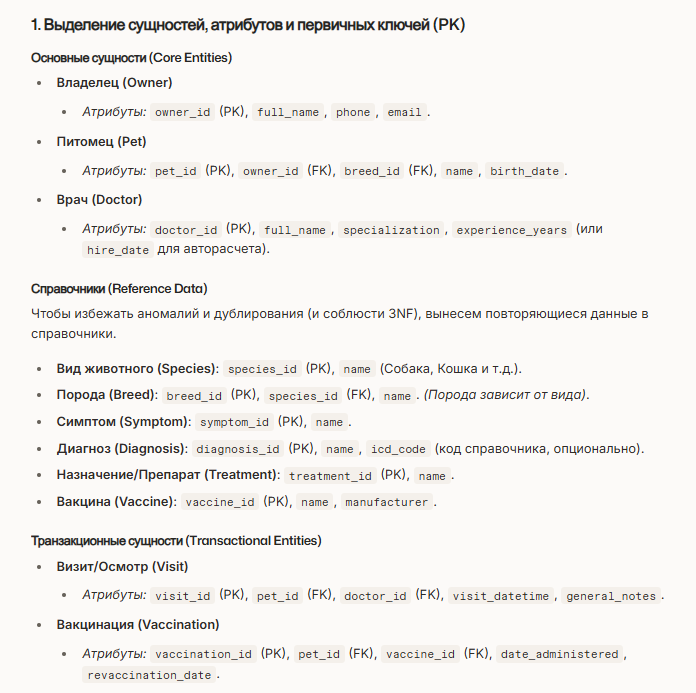
\includegraphics[width=17cm]{z5/1-1.png}
\end{figure}
\vspace{0.5em}
\begin{figure}[H]
\centering
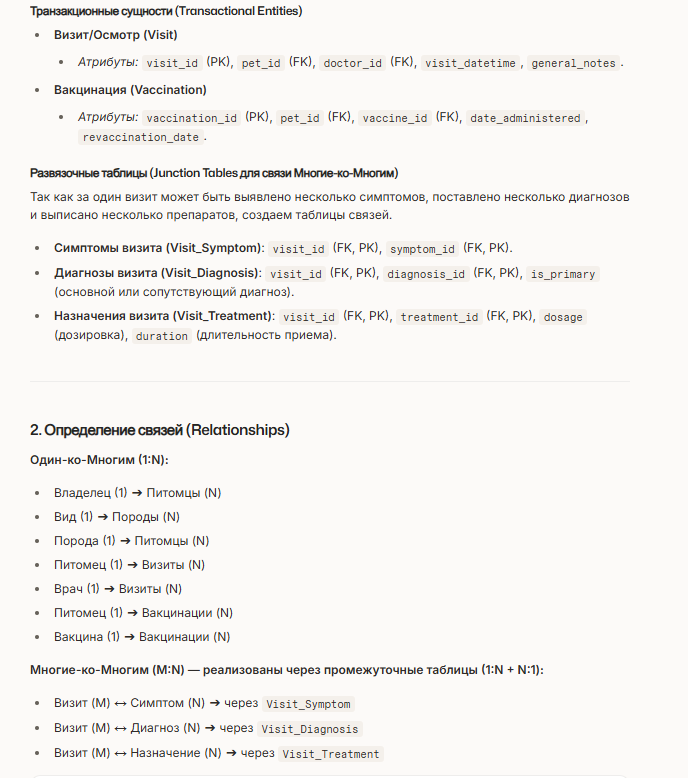
\includegraphics[width=17cm]{z5/1-1-1.png}
\caption{ч.1 (Выделение сущностей)}
\end{figure}
\vspace{0.5em}
\begin{figure}[H]
\centering
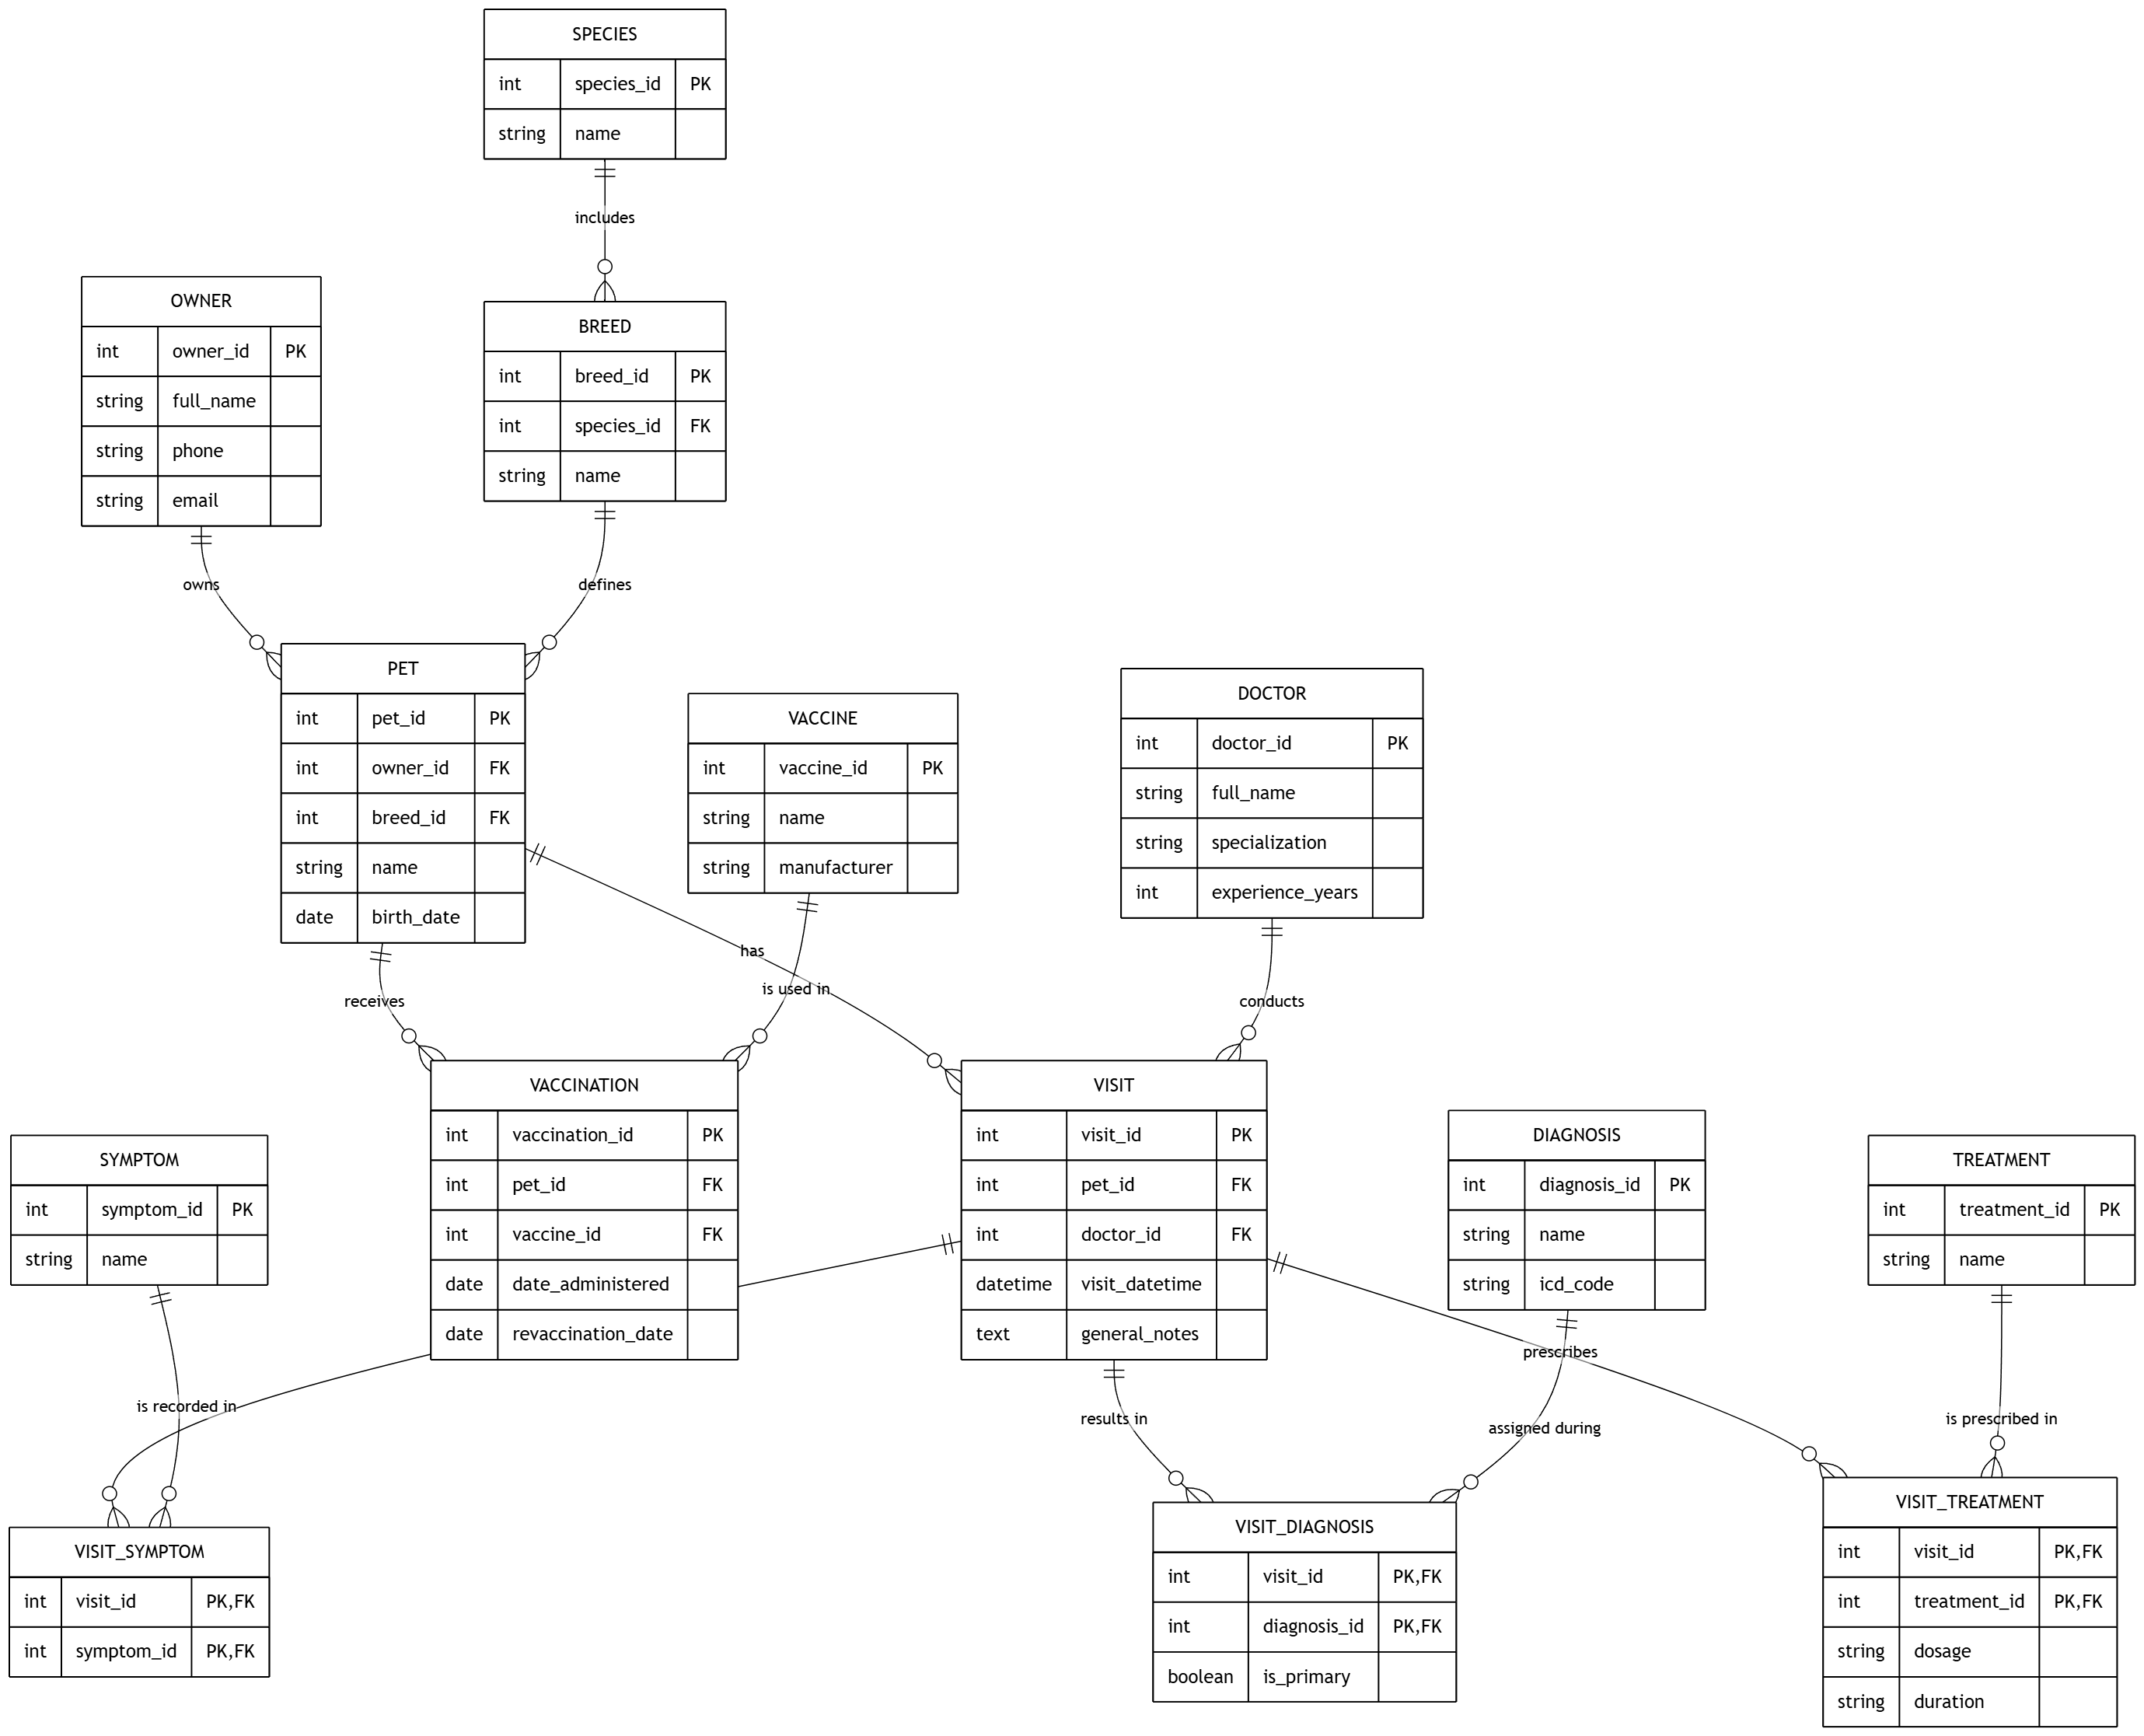
\includegraphics[width=17cm]{z5/1-2.png}
\caption{ч.2 (ER-диаграмма Mermaid)}
\end{figure}
\vspace{0.5em}
\begin{figure}[H]
\centering
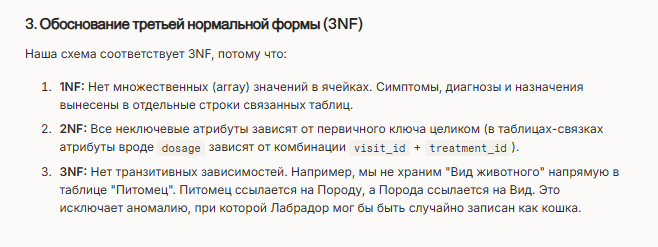
\includegraphics[width=17cm]{z5/1-3.png}
\caption{ч.3 (Проверка 3NF)}
\end{figure}
Анализ: Модель корректно разделила владельцев и питомцев, вынесла историю болезни в отдельную таблицу `medical\_visit`, избежав дублирования данных владельцев. Прививки связаны с питомцем и врачом. Схема соответствует 3NF.\\
\vspace{0.5em}
\textbf{Итерация 2 (генерация DDL-скрипта)}\\
Промпт:
\textit{
Отличная схема. Теперь сгенерируй DDL-скрипт для PostgreSQL. Требования:
\begin{itemize}
\item Явно укажи первичные и внешние ключи.
\item Добавь ограничения NOT NULL, UNIQUE, CHECK (например, phone формат, species IN (...)).
\item Для dates использовать DATE/TIMESTAMP с DEFAULT.
\item Все имена таблиц и полей в snake\_case.
\item При удалении владельца питомцы сохраняются, но владелец помечается как NULL (ON DELETE SET NULL).
\end{itemize}}
\vspace{0.5em}
Ответ модели:
\lstinputlisting[language=SQL]{z5/2.sql}
Анализ: Код корректен, использует современные стандарты PostgreSQL. Ограничения CHECK и каскадные правила расставлены логично.\\
\vspace{0.5em}
\textbf{Итерация 3 (генерация синтетических данных – few-shot)}\\
Промпт:
\textit{
Сгенерируй скрипт INSERT для наполнения таблиц тестовыми данными (минимум 4 владельца,
6 питомцев разных видов, 3 врача, 12 визитов, 10 прививок).
Используй реалистичные имена и даты. Сохрани логическую целостность FK.
Пример:
INSERT INTO owner (full\_name, phone, email) VALUES ('Иванов И.И.', '+79001234567', 'ivanov@mail.ru');
Продолжай в том же стиле.
}
\vspace{0.5em}
Ответ модели:
\lstinputlisting[language=SQL]{z5/3.sql}
Анализ: Данные семантически верны, FK ссылки валидны, даты распределены реалистично.\\
\vspace{0.5em}
\textbf{Итерация 4 (аналитические SQL-запросы)}\\
Промпт:
\textit{Составь три сложных аналитических запроса к этой БД:
\begin{enumerate}
\item Топ-5 самых часто посещаемых питомцев за последний год (по количеству визитов).
\item Для каждого врача: вычислить среднее количество дней между назначениями прививок,
используя оконные функции (LAG).
\item Скользящее среднее (moving average) количества визитов в клинике за последние 3 месяца
(по месяцам).
Используй JOIN, GROUP BY, HAVING и оконные функции (OVER, PARTITION BY, LAG, AVG).
\end{enumerate}}
\vspace{0.5em}
Ответ модели:
\lstinputlisting[language=SQL]{z5/4.sql}
Анализ: Запросы используют все требуемые конструкции. Второй запрос корректно применяет LAG для вычисления интервалов. Третий использует оконный AVG с ROWS BETWEEN.\\
\vspace{0.5em}
\textbf{Итерация 5 (анализ планов выполнения и оптимизация)}\\
Промпт:
\textit{Выступи в роли DBA. Проанализируй план выполнения запроса №1 (топ-5 питомцев).
Какие индексы ты предложишь добавить для ускорения? Напиши команды CREATE INDEX.
Укажи, можно ли переписать запрос эффективнее.}
\vspace{0.5em}
Ответ модели:
\begin{figure}[H]
\centering
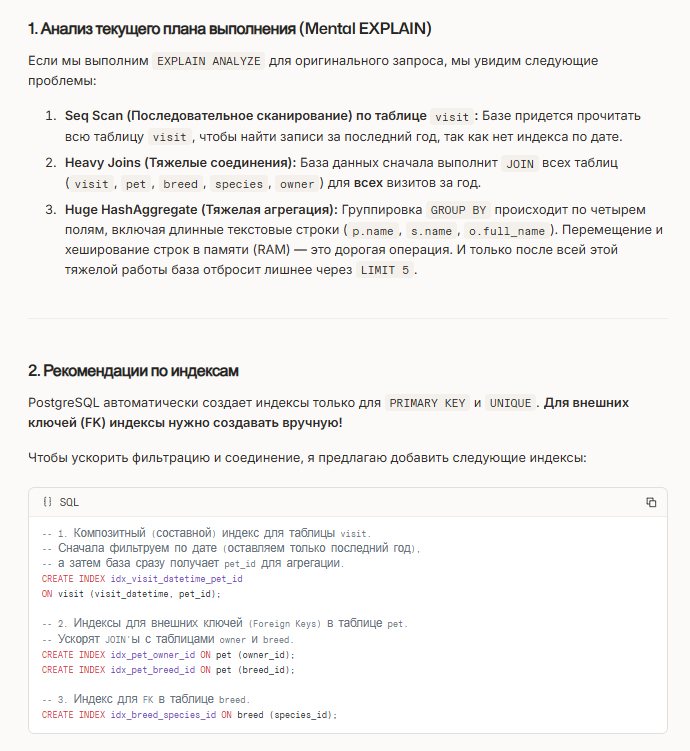
\includegraphics[width=17cm]{z5/5-1.png}
\end{figure}
\vspace{0.5em}
\begin{figure}[H]
\centering
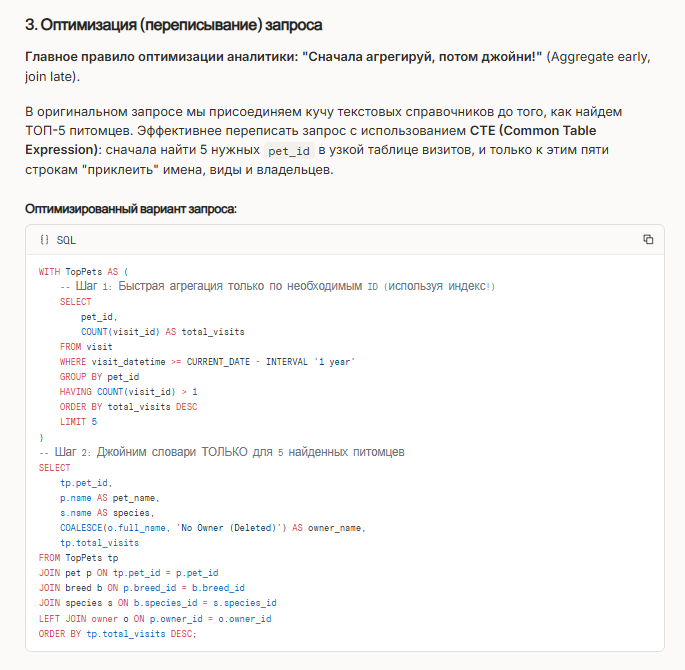
\includegraphics[width=17cm]{z5/5-2.png}
\end{figure}
\vspace{0.5em}
Анализ: Рекомендации точны. Предложены составные индексы на `medical\_visit(pet\_id, visit\_date)` и `vaccination(vet\_id, admin\_date)`. Объяснено влияние Sequential Scan vs Index Scan.

\subsection{Артефакты}
\begin{itemize}
\item ER-диаграмма – Mermaid-код и визуализация из Итерации 1.
\item DDL-скрипт – полный листинг из Итерации 2.
\item Синтетические данные – INSERT-скрипты из Итерации 3.
\item Аналитические запросы – три сложных запроса с оконными функциями из Итерации 4.
\item Рекомендации по индексам – из Итерации 5.
\end{itemize}
Все скрипты проверены в PostgreSQL 17, ошибок не возникло. Бизнес-данные возвращаются корректно, FK-целостность соблюдена.

\subsection{Сравнение моделей}
Финальный промпт (объединяющий все этапы) был подан контрольной модели DeepSeek R1 без изменений.
Результаты сравнения:
\begin{table}[h!]
\centering
\begin{tabular}{|l|p{5cm}|p{5cm}|}
\hline
\textbf{Критерий} & \textbf{модель (a)} & \textbf{модель (b)} \\
\hline
Нормализация (3NF) & 5 & 5 \\
\hline
Корректность SQL & 5 & 4 \\
\hline
Возврат бизнес-данных & 5 & 5 \\
\hline
Галлюцинации & нет & нет \\
\hline
\textbf{Итог} & 5.0 & 4.75 \\
\hline
\end{tabular}
\end{table}
Итог: Основная модель (a) точнее соблюдает синтаксис PostgreSQL (особенно в оконных функциях и работе с датами), корректно экранирует идентификаторы. Контрольная модель (b) предложила рабочую схему, но в третьем запросе допустила ошибку в синтаксисе `ROWS BETWEEN` (использовала `RANGE` без учета типов данных), что потребовало бы ручной правки. В целом обе модели справляются, но (a) выдает более продакшн-готовый код с первой итерации.

\subsection{Вывод}
Наиболее эффективными техниками промпт-инжиниринга оказались:
\begin{itemize}
\item \textbf{Ролевое моделирование} (Senior Data Architect, DBA) – задало строгий инженерный тон и предотвратило создание денормализованных таблиц.
\item \textbf{Цепочка рассуждений (CoT)} – последовательное прохождение этапов (ER $\rightarrow$ DDL $\rightarrow$ Данные $\rightarrow$ Запросы $\rightarrow$ Оптимизация) исключило потерю контекста и логические разрывы.
\item \textbf{Few-shot Prompting} – предоставление образца INSERT ускорило генерацию консистентных данных и устранило проблему «битых» FK-ссылок.
\end{itemize}
Задание подтвердило, что LLM способны самостоятельно проектировать нормализованные реляционные схемы и писать сложный аналитический SQL. Однако для критичных систем необходим контроль за типами данных, выбором индексов и валидацией оконных функций. Контрольная модель показала сопоставимый результат, но потребовала бы дополнительной итерации для исправления синтаксиса `OVER` в сложных агрегациях.